\documentclass[12pt]{article}
\usepackage[margin=1in]{geometry}
\usepackage{amsmath, amsthm, amssymb}
\usepackage[utf8]{inputenc}
\usepackage{amsmath}
\usepackage{graphicx}
\usepackage{hyperref}

\title{WebDB Project Plan}
\author{Phineas Callahan,Yuping Huang}
\begin{document}

 \maketitle

\section{The Data}
The datasets we are planning to use contain the results of all American congressional, gubernatorial and presidential 
elections. The data comes from CQ Press Voting and Elections Collection (\url{http://library.cqpress.com/elections/index.php}) in the form of CSV files. On the “Download Data” page 
(\url{http://library.cqpress.com/elections/download-data.php}),
one has to agree to the condition “these data are to be used for scholarly, educational, or personal use only” 
before proceeding to download. Henceforth academic use of the data should be permitted.

\section{The Audience}
The intended audience of this project (the data and the query interface) are those who are interested in electoral
politics, especially its evolution over time. Possible examples include researchers who want to understand historical voting trends in different
regions, students who are studying the change of voters' behaviors over time, political campaign managers who seek
to optimize their campaign strategy, and voters who are interested in the peformances of different parties and politicians
in the past.

\section{Functional\& Non-functional Requirements}
The WebDB project is conceived to have the following functional requirements:
\begin{enumerate}
 \item The system must store all the available congressional, gubernatorial and presidential data by county and congressional district from CQPress.
 \item The system must allow the users to select data based on locations and/or years.
 \item The system must provide appropriate visualizations for the selected dataset.
 \item The system must provide appropriate analytics for the selected dataset.
 \item The system must give users the option to retrive selected data (might be hard in terms of generating csv and the link to download)
\end{enumerate}

Besides, to support its functional requirements, we have specified the following non-functional requirements:
\begin{enumerate}
 \item The system must be accessible to users who are not able to manipulate a mouse.
 \item The UI must run cleanly and smoothly.
 \item The system must be accessible to users with restricted color vision.
\end{enumerate}

\section{Key Features}
The WebDB project should have the following features. The list is ordered in decsending priority. Time and resources
permitting, we aim to implement all of them.
\begin{enumerate}
 \item Navigation through a series of click-able maps.
 \item The ability to manually type in a query.
 \item Time series plotted, demonstrating how the nation, or its respective states and counties have changed their voting patterns over time.
 \item Pie charts breaking down election results for a requested year. 
 \item The ability to download data visualizations.
\end{enumerate}

\section{UI Mockup}
This project will be a single page web app that contains a landing page and the actual app itself. Two pdf's detailing the layout of these pages are included in the zip.
\hspace*{-1.5in}
\begin{figure}[p]
  \centering
 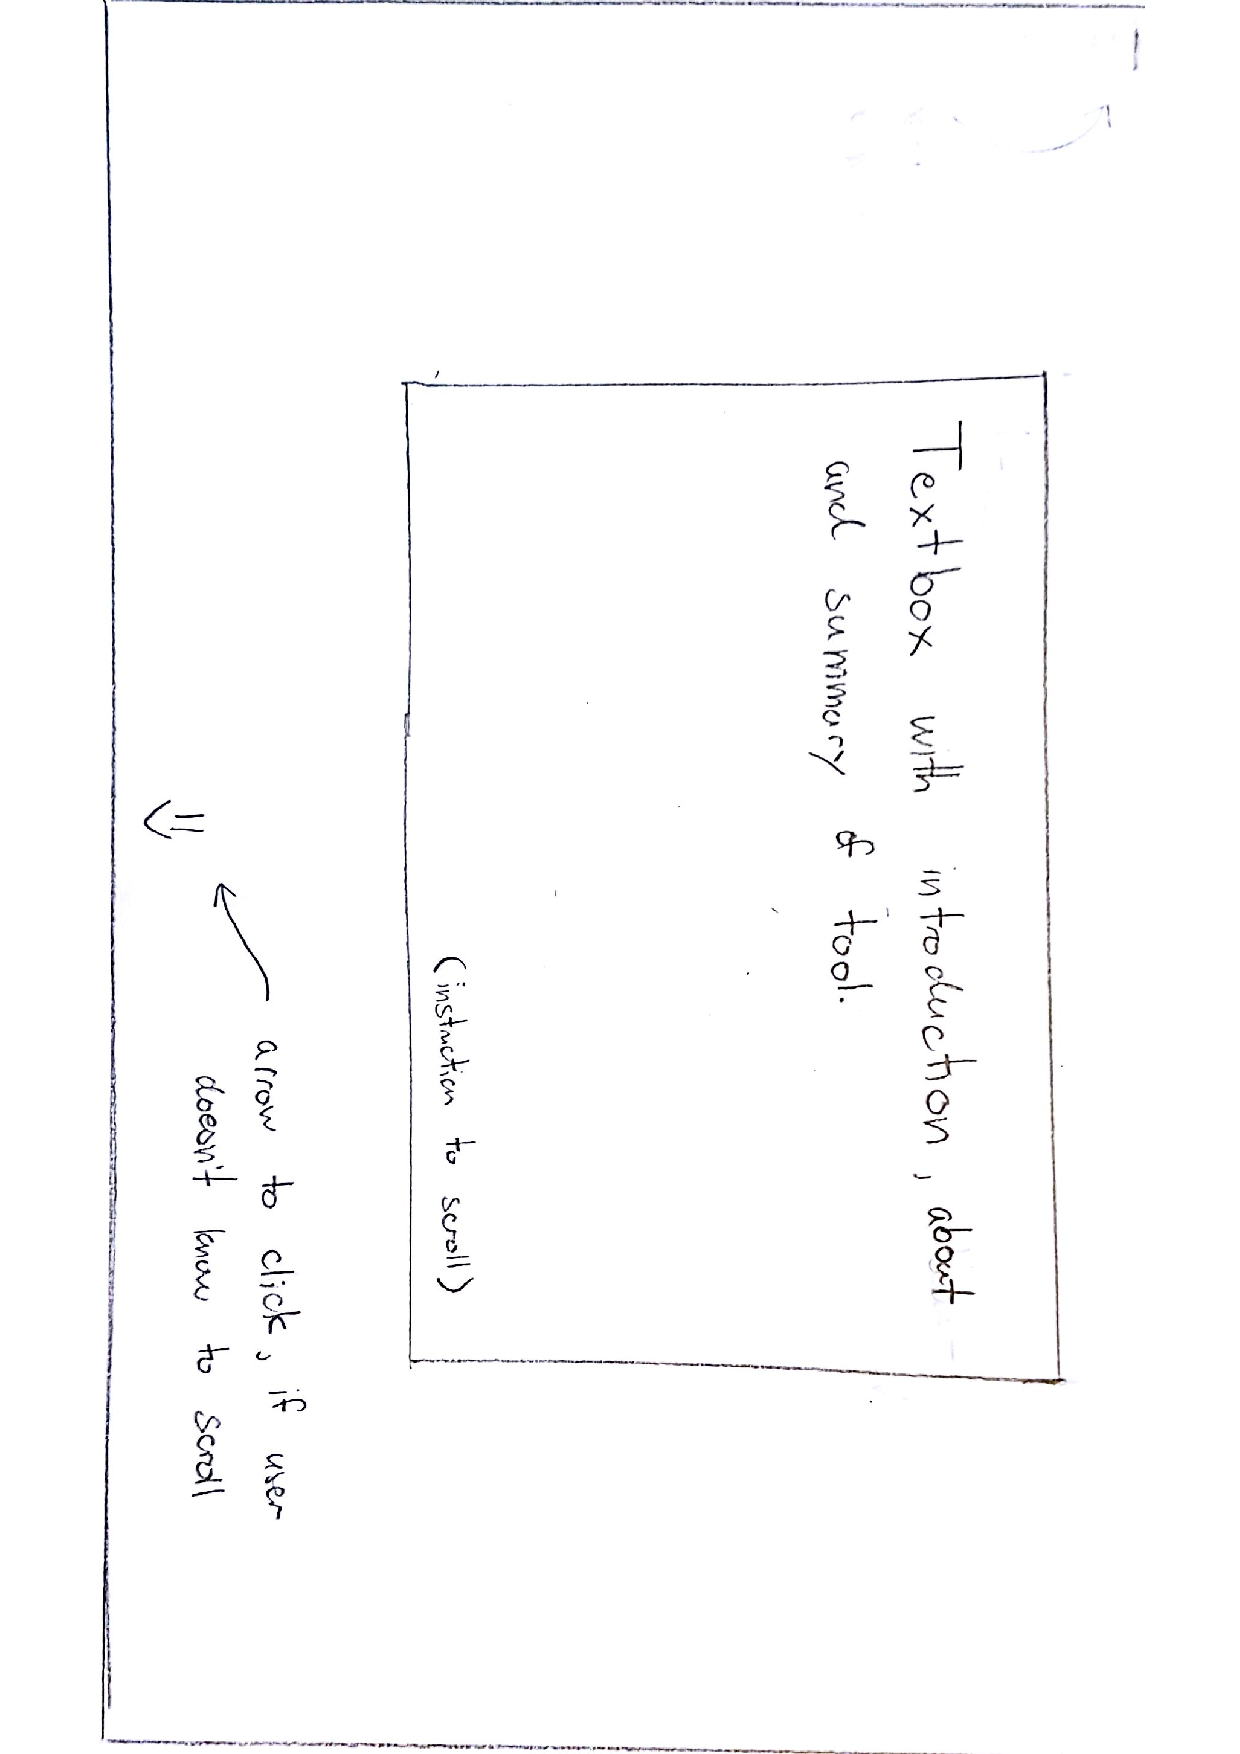
\includegraphics[width=0.4\textwidth,angle=90,origin=c,trim={0in 2in 2in 2in}]{HomepageUI.pdf}
 \caption{The landing page of the web app containing information about the app. User can either scroll down or click on the array to get to the app interface.}
\end{figure}
\begin{figure}[p]
  \centering
 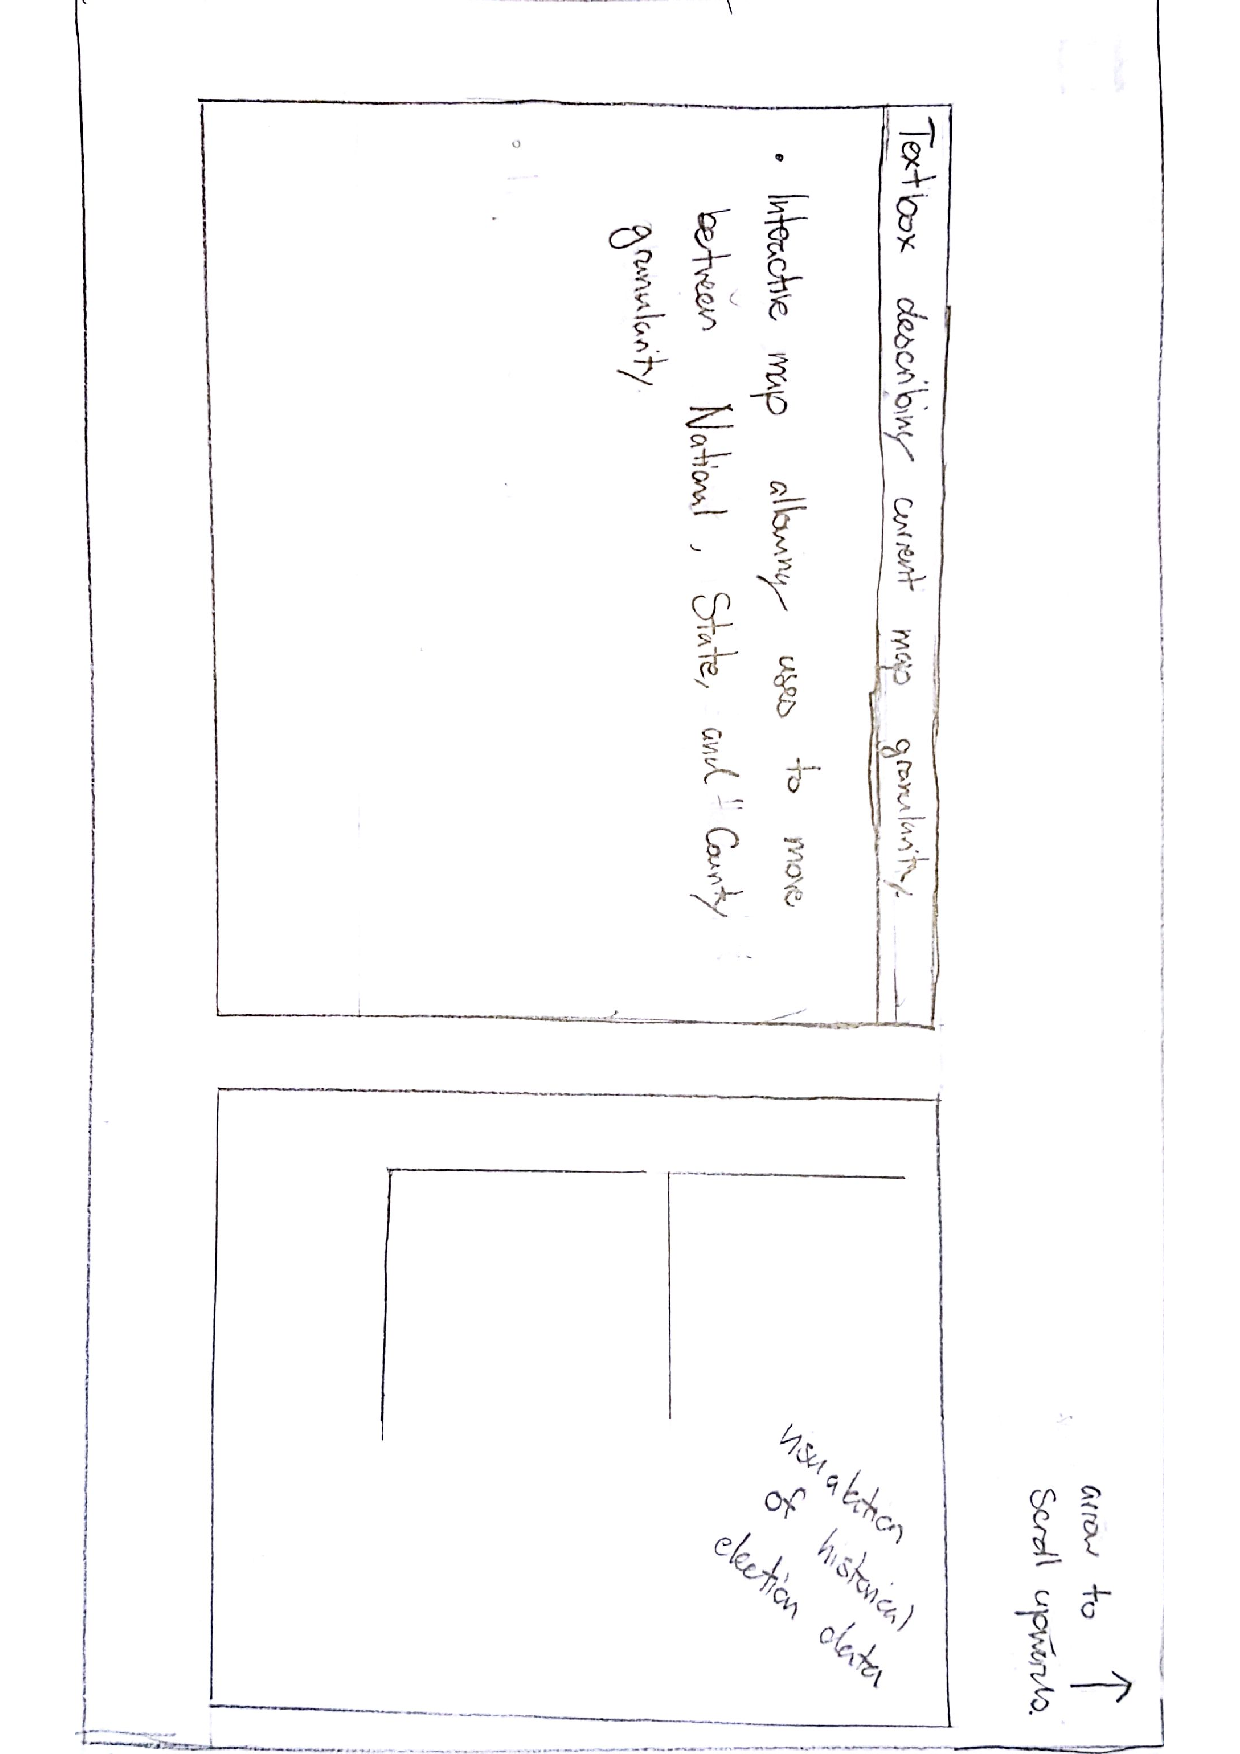
\includegraphics[width=0.4\textwidth,angle=90,origin=c,,trim={0in 2in 2in 2in}]{AppUI.pdf}
 \caption{The actual app interface. The main interface will be the interactive map and the user can type the year (range) in the text box area.
 The charts and analytics shows up in the right panel.}
\end{figure}

\end{document}
